\documentclass[draftthesis,tocnosub,noragright,centerchapter,12pt]{uiucecethesis09}

% Use draftthesis for notes and date markings on every page.  Useful when you
%   have multiple copies floating around.
% Use offcenter for the extra .5 inch on the left side. Needed with fullpage and fancy.
% Use mixcasechap for compatibility with hyperref package, which does NOT like all caps default
% Use edeposit for the adviser/committee on the title page.
% Use tocnosub to suppress subsection and lower entries in the TOC.
% PhD candidates use "proquest" for the proquest abstract.

\makeatletter

\usepackage{algorithm2e}
\usepackage[page]{appendix}
\usepackage{setspace}
\usepackage{epsfig}  % for figures
%\usepackage{graphicx}  % another package that works for figures
%\usepackage{subfigure}  % for subfigures
\usepackage{amsmath}  % for math spacing
%\usepackage{amssymb}  % for math spacing
%\usepackage{url}  % Hyphenation of URLs.
\usepackage{listings}
\usepackage{lscape}  % Useful for wide tables or figures.
\usepackage[justification=raggedright]{caption}	% makes captions ragged right - thanks to Bryce Lobdell
\usepackage{color}
\usepackage{tikz}
% \usetikzlibrary{arrows}
\usetikzlibrary{positioning}

\newif\ifsubmit
%\submittrue
\submitfalse
\ifsubmit

    \newcommand{\todo}[1]{}
    \newcommand{\tocite}[1]{}
    \newcommand{\outline}[1]{}
    \newcommand{\addtext}[1]{#1}
    \newcommand{\rmtext}[1]{}

\else

    \definecolor{commentColor}{rgb}{0.1, 0.6, 1.0}
    \definecolor{outlineColor}{rgb}{0.0, 0.50, 0.0}
    \definecolor{toCiteColor}{rgb}{0.5, 0.0, 0.5}
    \definecolor{addedColor}{rgb}{0.3, 0.5, 1.0}
    \definecolor{removedColor}{rgb}{0.8, 0.8, 0.8}

    \newcommand{\todo}[1]{[{\color{red}TODO: #1}]}
    \newcommand{\tocite}[1]{[{\color{toCiteColor}CITE: #1}]}
    \newcommand{\outline}[1]{[{\color{outlineColor}OUTLINE: #1}]}
    \newcommand{\addtext}[1]{{\color{addedColor}#1}}
    \newcommand{\rmtext}[1]{{\color{removedColor}\sout{#1}}}

\fi

% Uncomment the appropriate one of the following four lines:
\msthesis
%\phdthesis
%\otherdoctorate[abbrev]{Title of Degree}
%\othermasters[abbrev]{Title of Degree}

\title{System and Application Communication Modeling}
\author{Carl Pearson}
\department{Electrical and Computer Engineering}
\degreeyear{2018}

% Advisor name is required for
% - doctoral students for the ProQuest abstract
% - master's students who do not have a master's committee
\advisor{Wen-Mei Hwu}

% Uncomment the \committee command for
% - all doctoral students
% - master's students who have a master's committee
%\committee{Professor Firstname Lastname, Chair\\
%        Professor Firstname Lastname} % etc.

\begin{document}

%%%%%%%%%%%%%%%%%%%%%%%%%%%%%%%%%%%%%%%%%%%%%%%%%%%%%%%%%%%%%%%%%%%%%%%%%%%%%%%
% COPYRIGHT
%
%\copyrightpage
%\blankpage

%%%%%%%%%%%%%%%%%%%%%%%%%%%%%%%%%%%%%%%%%%%%%%%%%%%%%%%%%%%%%%%%%%%%%%%%%%%%%%%
% TITLE
%
\maketitle

%\raggedright
\parindent 1em%

\frontmatter

%%%%%%%%%%%%%%%%%%%%%%%%%%%%%%%%%%%%%%%%%%%%%%%%%%%%%%%%%%%%%%%%%%%%%%%%%%%%%%%
% ABSTRACT
%
\begin{abstract}
% Put the abstract in a file called "abs.tex" and it'll be inputted here.
With the end of dennard scaling, high-performance computing increasingly relies on heterogeneous systems with specialized hardware to improve application performance.
This trend has driven up the complexity of high-performance software development, as developers must manage multiple programming systems and develop system-tuned code to utilize specialized hardware.
In addition, it has exacerbated existing challenges of data placement as the specialized hardware often has local memories to fuel its computational demands.
In addition to using appropriate software resources to target application computation at the best hardware for the job, application developers now much manage data movement and placement within their application, which also must be specifically tuned to the target system.
Instead of relying on the application developer to have specialized knowledge of system characteristics and specialized expertise in multiple programming systems, this work proposes a heterogeneous system communication library that automatically choses data location and data movement for high-performance application development and execution on heterogeneous systems.
This work presents the foundational components of that library: a systematic approach for characterization of system communication links and application communication demands.
\end{abstract}


%%%%%%%%%%%%%%%%%%%%%%%%%%%%%%%%%%%%%%%%%%%%%%%%%%%%%%%%%%%%%%%%%%%%%%%%%%%%%%%
% DEDICATION
%
\begin{dedication}
% Whatever dedication you want.
To my family, for their love and support.
\end{dedication}

%%%%%%%%%%%%%%%%%%%%%%%%%%%%%%%%%%%%%%%%%%%%%%%%%%%%%%%%%%%%%%%%%%%%%%%%%%%%%%%
% ACKNOWLEDGMENTS
%
% Put acknowledgments in a file called "ack.tex" and it'll be inputted here.
\begin{acknowledgments}
I would like to thank Professor Wen-Mei Hwu.

I would also like to thank the members of the IMPACT group for their continual support.
\end{acknowledgments}

%%%%%%%%%%%%%%%%%%%%%%%%%%%%%%%%%%%%%%%%%%%%%%%%%%%%%%%%%%%%%%%%%%%%%%%%%%%%%%%
% TABLE OF CONTENTS
%
\tableofcontents

%%%%%%%%%%%%%%%%%%%%%%%%%%%%%%%%%%%%%%%%%%%%%%%%%%%%%%%%%%%%%%%%%%%%%%%%%%%%%%%
% LIST OF TABLES
%
% The List of Tables is not strictly necessary. Omitting the List of Tables will
% simplify the thesis check and reduce the number of corrections.
\listoftables

%%%%%%%%%%%%%%%%%%%%%%%%%%%%%%%%%%%%%%%%%%%%%%%%%%%%%%%%%%%%%%%%%%%%%%%%%%%%%%%
% LIST OF FIGURES
%
% The List of Figures is not strictly necessary. Omitting the List of Figures will
% simplify the thesis check and reduce the number of corrections.
\listoffigures

%%%%%%%%%%%%%%%%%%%%%%%%%%%%%%%%%%%%%%%%%%%%%%%%%%%%%%%%%%%%%%%%%%%%%%%%%%%%%%%
% LIST OF ABBREVIATIONS
%
% The List of Abbreviations is not strictly necessary.
\chapter{LIST OF ABBREVIATIONS}

%\begin{symbollist*}
%\item[EPIC] Explicitly Parallel Instruction Computing
%\item[GPU] Graphics Processing Unit
%\item[VLIW] Very Long Instruction Word
%\end{symbollist*}


%%%%%%%%%%%%%%%%%%%%%%%%%%%%%%%%%%%%%%%%%%%%%%%%%%%%%%%%%%%%%%%%%%%%%%%%%%%%%%%
% LIST OF SYMBOLS
%
%\begin{symbollist}[0.7in]
%\item[$\tau$] Time taken to drink one cup of coffee.
%\end{symbollist}

\mainmatter

%%%%%%%%%%%%%%%%%%%%%%%%%%%%%%%%%%%%%%%%%%%%%%%%%%%%%%%%%%%%%%%%%%%%%%%%%%%%%%%
% INSERT REAL CONTENT HERE
%

%\include{intro}	% for INTRODUCTION in "intro.tex"
%\include{exper}
%\include{concl}

\chapter{Introduction}
Add a citation~\cite{IEEEexample:urlsty} to make the build not fail.

The first chapter should introduce the problem studied and describe the main results obtained in the thesis.
In order to provide guidance to the reader, the first chapter should briefly describe the organization of the rest of the thesis.
The first chapter can also give the background of previous work on the subject and the method used in attacking the problem.
\chapter{Background}


%
%
%
\section{Communication Links}

\subsection{PCI}
\subsection{NVLink}
\subsection{QPI}
\subsection{X bus}
\subsection{CAPI}

%
%
%
\section{Programming Systems}
\subsection{CUDA}
\label{sec:cuda}


CUDA Unified Memory~\cite{harris2013cudaunifiedmemory} provides a single pool of memory that is accessible from the CPU and GPU by a single pointer.
CUDA automatically migrates data between the physically distinct CPU and GPU memory as needed, allowing GPU kernels to access the memory as if it were in the global memory, and CPU functions to access the memory as if it were in the system memory.
This simplifies the programming model.

\todo{unified memory peer access}

\subsection{HSA}
\label{sec:hsa}


%
%
%
\section{Profiling Tooling}

\subsection{CUDA Profiling Tools Interface}
\label{sec:cupti}

The CUDA Profiling Tools Interface~\cite{nvidia2017cupti} (CUPTI) ``provides...detailed information about how applications are using the GPU in a system.''
Users may inject code into the entry and exit point of every CUDA C Runtime and CUDA Driver API function call.
Additionally, users may configure and query hardware and software event counters to get insight into the operation of the GPU and CUDA stack.
The event counters include instruction count, instruction throughput, memory loads/stores, memory throughput, cache hits/misses, branches and custom profile triggers.
Chapter~\ref{ch:app-char} describes how \todo{hwcomm-apptracer} uses CUPTI to record memory allocations, kernel arguments, and timestamps to build a model of the application execution.

\subsection{\texttt{LD\_PRELOAD}}
\label{sec:ldpreload}

LD\_PRELOAD~\cite{kerrisk2017ld} is a mechanism by which the ld linker will load additional user-specific shared objects before any others.
If a function definition is present in a pre-loaded shared object, it will override the implementation present in later objects.
When combined with dlsym()~\cite{kerrisk2017dlysm}, it can be used to inject code into the entry of library calls in dynamically-linked binaries.
Chapter~\ref{ch:app-char} describes how \todo{hwcomm-apptracer} uses LD\_PRELOAD to record special information about cuBLAS and cuDNN calls.

\cite{kerrisk2017ld}


\chapter{System Characterization}
\label{ch:sys-char}

High-performance data movement in heterogeneous systems requires information about the properties of the communication links between system storage and compute components.
Although specifications of system components are often available\todo{cite some examples}, the real-world properties of these links depends on how applications use the links, and whether or not the links are shared between system components.
\todo{For example, Figure~\ref{fig:actual-perf} shows modeled and achieved cuda memcpy bandwidth.}
With full knowledge of link properties it is possible to derive an accurate model of link performance, that approach has two key barriers
\begin{itemize}
    \item Detailed link hardware properties are not available, e.g., when the link provides a competitive advantage for an OEM.
    \item Detailed link software properies are not available, e.g., when the drivers are proprietary.
    \item Even if a link is pysically present on the system, it may not be available to the application {e.g., due to bugs in the system configuration}
\end{itemize}
Instead of deriving a model of link performance from the ``first principles'' of link properties, this work attempts to generate an empirical model of performance of data movement in the system.

Though data movement between many different system components is possible, this work focuses on CPU-CPU and CPU-GPU data transfers.
Section~\ref{sec:system-model} describes an overview of the system model.
Section~\ref{sec:topology-exploration} describes a method for discovering data sources, sinks, and communication paths in a system.
Section~\ref{sec:link-char} describes the approach to characterize communication links.

\begin{figure}[ht]
    \centering
    \includegraphics[width=0.5\textwidth,draft]{../figures/actual-cuda-memcpy.png}
    \caption[\todo{short}]{\todo{long}}
    \label{fig:actual-cuda-memcpy}
\end{figure}

\section{System Model}
\label{sec:system-model}

The harware system is represented by a graph $G_s = \{E,V\}$ where $E$ is a set of edges representing communication links, and $V$ is a set of vertices representing data sources/sinks.
Sections~\ref{sec:system-vertices} and \ref{sec:system-edges} describe the specific system components explored.
Associated with each edge is a performance model function $M: C,U \rightarrow P$ that maps a communication pattern $C$ and a link utilization $U$ to an achievable performance $P$.

The communication pattern $P$ has the following parameters:
\begin{itemize}
    \item The communication API or method used (e.g., \texttt{fread()}, CUDA unified memory page transfer).
    \item The number, size, and priority of pending transfers on the link.
\end{itemize}

The link utilization $U$ a set of extant communication patterns already sharing the link, separate from the communication of interest $C$.



Each vertex in $V$ represents a data source/sink.



%
% SECTION
%
\section{Topology Exploration}
\label{sec:topology-exploration}

The topology exploration is done in several phases:

\begin{minipage}[ht]{\textwidth}
\begin{enumerate}
    \item Enumerate and link CPU sockets
    \item Enumerate PCI devices
    \item Update GPUs to NVIDIA GPUs as appropriate
    \item Enumerate Linux block devices
\end{enumerate}
\end{minipage}

First, the Portable Hardware Locality~\cite{broquedis2010hwloc} (hwloc) library is used to enumerate the present CPU sockets.
As the test systems only have two sockets, all discovered sockets are considered to be directly connected by an SMP bus.
Next, hwloc is used to descend through the PCI device tree and connect all PCI devices with PCI links of the appropriate type.
Next, the NVIDIA Management Library~\cite{nvidia2017nvml} (NVML) is used to enumerate all NVIDIA GPUs.
Those GPUs are matched by PCI address with previously-discovered PCI devices and information about those GPUs is added to $G_s$.
NVML is then used to discover whether NVLink is supported on each GPU, and which device the NVLink terminates at.
Finally, linux block devices are enumerated through \todo{more detail} and added to $G_s$.
Where applicable, enough information about the device is stored within the vertex to be able to access the device later.

\subsection{Vertex Types}
\label{sec:system-vertices}

Table~\ref{tab:topology-vertices} summarizes the discoverable types of data sources and sinks investigated by this work.


\begin{table}[]
    \centering
    \caption[Discoverable vertex types]{\todo{long caption}}
    \label{tab:topology-vertices}
    \begin{tabular}{|c|c|}
    \hline
    \textbf{Vertex Type}    & \textbf{Description} \\ \hline
    CPU Socket              &                      \\ \hline
    PCI Device              &                      \\ \hline
    PCIe Hostbridge         &                      \\ \hline
    PCIe Bridge             &                      \\ \hline
    CUDA GPU                &                      \\ \hline
    Linux Block Device      &                      \\ \hline
    Linux Network Interface &                      \\ \hline
    \end{tabular}
\end{table}

\subsection{Edge Types}
\label{sec:system-edges}

In $G_s$, the vertices are connected by the discoverable edge types shown in Table~\ref{tab:topology-edges}.

\begin{table}[]
    \centering
    \caption[Discoverable edge types]{\todo{long caption}}
    \label{tab:topology-edges}
    \begin{tabular}{|c|c|}
    \hline
    \textbf{Edge Type} & \textbf{Description} \\ \hline
    SMP Bus            &                      \\ \hline
    PCIe Bus           &                      \\ \hline
    NVLink             &                      \\ \hline
    SATA Bus           &                      \\ \hline
    \end{tabular}
\end{table}



%
% SECTION
%
\section{Link Characterization}
\label{sec:link-char}

After the system graph $G_s$ has been generated, the next task is to characterize the communication capabilities of the system.
The goal of this characterization is to determine the rate at which data of a particular size can be moved between devices.
Ideally, this characterization would occur on a per-link basis along each available path between two communicating devices.
In practice, the communication between many devices is mediated by APIs exposed by the operating system or vendor library.
These APIs abstract away some complexity from the data movement.

\begin{figure}
    \centering
    \begin{tikzpicture}[
        cpunode/.style={circle, draw=green!60, fill=green!5, very thick, minimum size=7mm},
        gpunode/.style={rectangle, draw=red!60, fill=red!5, very thick, minimum size=5mm},
        blocknode/.style={rectangle, draw=red!60, fill=red!5, very thick, minimum size=5mm},
        ]
        %Nodes
        \node[cpunode]   (s0)                  {Socket0};
        \node[blocknode] (b0)    [below=of s0] {Disk0};
        \node[cpunode]   (s1)    [right=of s0] {Socket1};
        \node[gpunode]   (g0)    [below=of s1] {GPU0};

        %Lines
        \path[-] (s0.east)  edge node [above] {SMP}    (s1.west);
        \path[-] (s0.south) edge node [left]  {PCIe0}  (b0.north);
        \path[-] (s1.south) edge node [right] {PCIe1}  (g0.north);
    \end{tikzpicture}
    \caption[A simple example topology]{\todo{clean this up}\todo{long caption}}
    \label{fig:simple-topology}
\end{figure}

For example, consider the simple example system topology in Figure~\ref{fig:simple-topology}.
If a CPU thread running on CPU1 calls \texttt{fread()} to move a block of data from Disk0 to the memory associated with CPU1, the OS will transparently move that data along the PCIe0 and SMP0 links.
Since this capability is exposed to applications, it is useful to characterize it as well, not just the intermediate PCIe0 and SMP links.

An overview of the characterization algorithm is shown in Algorithm~\ref{alg:link-char}.

\begin{algorithm}[ht]
    \SetAlgoLined
    \KwResult{Characterization of all links between all vertices in $G_s$ }
     Build $G_s$ as described in Section~\ref{sec:topology-exploration}\;
     \For{$v_1$ in $V$}{
         \For{$v_2$ in $V$}{
             \If{$v_1 \ne v_2$}{
                Chars $\gets$ SupportedCharacterizers($v_1$,$v_2$)\;
                \For{c in Chars} {
                    c($v_1$, $v_2$)\;
                }
             }
         }
     }
     \caption{Link characterization.}
     \label{alg:link-char}
\end{algorithm}

For each pair of vertices, \todo{hwcomm} determines whether direct communication between those vertices is supported by the operating system or vendor libraries.
For vertices with a path of more than one link between them (e.g. Disk0 to Socket1 in Figure~\ref{fig:simple-topology}) those individual links will be characterized separately.
For vertices with multiple paths between them, the characterized path will be implicitly chosen by the applied characterization method.

\subsubsection{CUDA \texttt{cudaMemcpy} with Pinned Memory}

This characterization method outlined in Algorithm~\ref{alg:cuda-h2d} is available for paths terminated by a CPU socket and a CUDA GPU.
A pinned memory allocation on the host and corresponding GPU memory allocation on the GPU are established.
Bandwidth betwene host and devices achieved at various transfer sizes is established by copying various amounts of data between the memory allocations.

\begin{algorithm}[ht]
    \SetAlgoLined
    \KwResult{bandwidth vs. transfer size between socket $s$ and CUDA GPU $g$}
    bind CPU thread to $s$\;
    bind memory allocation to $s$\;
    poolSize $\gets$ $\frac{gpuMemory}{2}$\;
    socketPool $\gets$ \texttt{cudaMallocHost(poolSize)}\;
    gpuPool $\gets$ \texttt{cudaMalloc(poolSize)}\;
    \For{transferSize := $1$ to poolSize}{
        start $\gets$ wall\_time()\;
        \eIf{direction == deviceToHost} {
            \texttt{cudaMemcpy(socketPool, gpuPool, transferSize, cudaMemcpyHostToDevice)}\;
        }{
            \texttt{cudaMemcpy(gpuPool, socketPool, transferSize, cudaMemcpyHostToDevice)}\;
        }
        stop $\gets$ wall\_time()\;
        bandwidth $\gets$ $\frac{copySize}{stop - start}$\;
    }
    \caption{CUDA cudaMemcpy with pinned memory.}
    \label{alg:cuda-h2d}
\end{algorithm}

\subsubsection{CUDA \texttt{cudaMemcpy} between CUDA GPUs}

This characterization method outlined in Algorithm~\ref{alg:cuda-d2d} is available for paths terminated by a CUDA GPU on both ends.
A GPU memory allocation is established on each GPU.
Bandwidth achieved at various transfer sizes between GPUs is established by copying various amounts of data between the memory allocations.

\begin{algorithm}[ht]
    \SetAlgoLined
    \KwResult{bandwidth vs. transfer size between CUDA GPUs $g_0$ and $g_1$}
    poolSize $\gets$ $\frac{gpuMemory}{2}$\;
    gpu0Pool $\gets$ \texttt{cudaMalloc(poolSize)}\;
    gpu1Pool $\gets$ \texttt{cudaMalloc(poolSize)}\;
    \For{transferSize := $1$ to poolSize}{
        start $\gets$ wall\_time()\;
        \texttt{cudaMemcpy(gpu1Pool, gpu0Pool, transferSize, cudaMemcpyDeviceToDevice)}\;
        stop $\gets$ wall\_time()\;
        bandwidth $\gets$ $\frac{copySize}{stop - start}$\;
    }
    \caption{CUDA cudaMemcpy between CUDA GPUs}
    \label{alg:cuda-d2d}
\end{algorithm}

\subsubsection{CUDA \texttt{memcpyPeer}}

This characterization method outlined in Algorithm~\ref{alg:cuda-d2d} is available for paths terminated by a CUDA GPU on both ends.
A GPU memory allocation is established on each GPU.
Bandwidth between GPUs achieved at various transfer sizes is established by copying various amounts of data between the memory allocations.

\begin{algorithm}[ht]
    \SetAlgoLined
    \KwResult{bandwidth vs. transfer size between CUDA GPUs $g_0$ and $g_1$}
    poolSize $\gets$ $\frac{gpuMemory}{2}$\;
    gpu0Pool $\gets$ \texttt{cudaMalloc(poolSize)}\;
    gpu1Pool $\gets$ \texttt{cudaMalloc(poolSize)}\;
    \For{transferSize := $1$ to poolSize}{
        start $\gets$ wall\_time()\;
        \texttt{cudaMemcpyPeer(gpu1Pool, gpu0Pool, transferSize)}\;
        stop $\gets$ wall\_time()\;
        bandwidth $\gets$ $\frac{copySize}{stop - start}$\;
    }
    \caption{CUDA cudaMemcpy between CUDA GPUs}
    \label{alg:cuda-p2p}
\end{algorithm}

\todo{The difference between this and cudaMemcpy(cudaMemcpyDeviceToDevice)}

\subsubsection{CUDA Unified Memory}

This characterization method outlined in Algorithm~\ref{alg:cuda-d2d} is available for path terminated by CUDA-supported devices on both ends.
A single unified memory allocation is established, and the entire allocation is touched by the source device to ensure the data is resident on that device.
Bandwidth between devices under various access patterns is established by executing a kernel with the corresponding pattern on the destination device.

\textbf{Linear Pattern}

\todo{description}

\textbf{Random Pattern}

\todo{description}


\subsubsection{OpenMP Socket to Socket Bandwidth}

The symmetric multi-processing links between CPU sockets are characterized by a synthetic workload generated using OpenMP~\cite{openmp2013}.
This workload creates multiple threads reading remote data in an attempt to saturate the socket memory controllers and SMP bus.
Algorithm~\ref{alg:h2h} describes the approach.

\begin{algorithm}[ht]
    \SetAlgoLined
    \KwResult{bandwidth vs. transfer size between CPU sockets $src$ and $dst$}
    numThreads $\gets$ 10\;
    \todo{Choice of elemSize}\;
    \For{poolSize $\gets$ 128 to sweepFinish} {
        bind process to $src$\;
        bind memory allocation to $src$\;
        \For{tid $\gets$ 0 := numThreads}{
            regions[tid] $\gets$ alloc(poolSize)\;
        }
        bind process to $dst$\;
        start OpenMP parallel region\;
        start $\gets$ wall\_time()\;
        \texttt{sum\_array(region[omp\_get\_thread\_num(), elemSize])}\;
        stop $\gets$ wall\_time()\;
        bandwidth $\gets$ $\frac{copySize}{stop - start}$\;
    }
    \caption{Synthetic workload for testing SMP bus.}
    \label{alg:h2h}
\end{algorithm}

\texttt{sum\_array()} is a function used to ensure that every data element is accessed, and the compiler does not optimize out the otherwise unused remote data read.
\texttt{sum\_array()} adds the elements in the region using loads and accumulates of a desired size.

%
% SECTION
%
\section{System Characterization Case Studies}

The system characterization was executed on two high-performance heterogeneous systems: an IBM S822LC ``Minsky''~\cite{ibm2015minsky}, and an NVIDIA DGX-1~\cite{nvidia2016dgx1}.
The two systems both feature 512 GB of system memory, two multi-core GPUs, and multiple NVIDIA Tesla P100 GPUs.
Their key differences are in CPU architecture (ppc64le for ``Minsky'', x86-64 for DGX-1), number of GPUs (4 vs 8), and GPU connection topology (bonded NVLink vs hybrid PCIe/NVLink).

\subsection{IBM S822LC ``Minsky''}
\label{sec:topology-minsky}

The IMB ``Minsky'' machine consists of two symmetric sections, connected by an IBM X bus between two 10-core Power8+ CPUs with 8-way simultaneous multithreading (SMT).
Each CPU is connected to 256GB of DDR3 RAM.
Each CPU is also connected to two NVIDIA Tesla P100 GPUs by two bonded NVLink blocks.
Those P100s within the symmetric section are also connected to each other by two bonded NVLinks.
The second CPU socket hosts the majority of the PCI devices on the system, including the network interfaces and the disks.
Figure \ref{fig:topo-minsky-simple} shows a simplified view\footnote{Figure \ref{fig:topo-minsky-actual} shows a detailed view.} of the topology discovered by \todo{hwcomm}.


\begin{figure}
    \centering
    \begin{tikzpicture}[
        cpunode/.style={circle, draw=green!60, fill=green!5, very thick, minimum size=7mm},
        gpunode/.style={rectangle, draw=red!60, fill=red!5, very thick, minimum size=5mm},
        blocknode/.style={rectangle, draw=red!60, fill=red!5, very thick, minimum size=5mm},
        nvlink/.style={double distance=3pt},
        ]
        %Nodes
        \node[cpunode]   (s0)                  {Socket0};
        \node[cpunode]   (s1)    [right=of s0] {Socket1};
        \node[gpunode]   (g0)    [below=of s0] {GPU0};
        \node[gpunode]   (g1)    [left=of g0]  {GPU1};
        \node[gpunode]   (g2)    [below=of s1] {GPU2};
        \node[gpunode]   (g3)    [right=of g2] {GPU3};

        %Lines
        \path[-] (s0.east)  edge node [above] {SMP}    (s1.west);

        \path[<->] (s0.south) edge [nvlink] node [left]  {NVLink}  (g0.north);
        \path[<->] (s0.west)  edge [nvlink] node [left]  {NVLink}  (g1.north);
        \path[<->] (g0.west)  edge [nvlink] node [below] {NVLink}  (g1.east);

        \path[<->] (s1.south) edge [nvlink] node [left]  {NVLink}  (g2.north);
        \path[<->] (s1.east)  edge [nvlink] node [right] {NVLink}  (g3.north);
        \path[<->] (g2.east)  edge [nvlink] node [below] {NVLink}  (g3.west);
    \end{tikzpicture}
    \caption{IBM ``Minsky'' simplified topology.}
    \label{fig:topo-minsky-simple}
\end{figure}


\subsection{NVIDIA DGX-1}
\label{sec:topology-dgx1}

The NVIDIA DGX-1 machine consists of two symmetric sections.
Each section consists of one 20-core Intel Xeon E5-2698v4 CPUs with 2-way SMT.
Each CPU is connected to 256GB of DDR4 RAM.
Each section has 4 NVIDIA Tesla P100 GPUs coupled by single NVLinks.
The sections are connected by an Intel QPI bus between the CPUs, as well as NVLinks between corresponding GPUs.
The first CPU socket hosts the majority of the PCI devices on the system, including the network interfaces and the disks.
Figure \ref{fig:topo-dgx-simple} shows a simplified view\footnote{Figure ~\ref{fig:topo-dgx-actual} shows a detailed view.} of the topology discovered by \todo{hwcomm}.


\begin{figure}
    \centering
    \begin{tikzpicture}[
        cpunode/.style={circle, draw=green!60, fill=green!5, very thick, minimum size=7mm},
        gpunode/.style={rectangle, draw=red!60, fill=red!5, very thick, minimum size=5mm},
        blocknode/.style={rectangle, draw=red!60, fill=red!5, very thick, minimum size=5mm},
        ]
        %Nodes
        \node[cpunode]   (s0)                  {Socket0};
        \node[blocknode] (b0)    [below=of s0] {Disk0};
        \node[cpunode]   (s1)    [right=of s0] {Socket1};
        \node[gpunode]   (g0)    [below=of s1] {GPU0};

        %Lines
        \path[-] (s0.east)  edge node [above] {SMP}    (s1.west);
        \path[-] (s0.south) edge node [left]  {PCIe0}  (b0.north);
        \path[-] (s1.south) edge node [right] {PCIe1}  (g0.north);
    \end{tikzpicture}
    \caption{NVIDIA DGX-1 simple topology.}
    \label{fig:topo-dgx-simple}
\end{figure}
\chapter{Application Characterization}

\section{Application Model}

Graph $G_a$...

\section{Application Monitoring}

Using CUPTI~\cite{nvidia2017cupti} and \texttt{LD\_PRELOAD}~\cite{kerrisk2017ld}.

\section{Application Modeling Case Studies}
\subsection{Chai}
\subsection{Caffe}
\subsection{Graph Challenge}
\subsection{Lulesh}
\chapter{Performance Modeling}
\label{ch:performance}

\section{Methodology}

The system graph $G_s$ and the application graph $G_a$ have analogous structure, summarized in Table~\ref{tab:graph-comparison}.

\begin{table}[h]
    \centering
    \caption{Analogous graph component roles in $G_a$ and $G_s$.}
    \label{tab:graph-comparison}
    \begin{tabular}{|c|c|c|}
    \hline
    \textbf{Graph Component} & \multicolumn{2}{|c|}{\textbf{Meaning in Graph}}   \\ \hline
                             & $\bm{G_a}$    & $\bm{G_s}$                        \\ \hline \hline
    \textbf{Vertex}          & Data source or sink & compute or storage hardware \\ \hline
    \textbf{Edge}            & Data transfer & communication link                \\ \hline
    \end{tabular}
\end{table}



\section{\{Minsky, DGX\} $\times$ \{Applications\}}
\chapter{Related Work}

\section{System Topology Enumeration}

hwloc~\cite{broquedis2010hwloc} provides a tree of system components, while modern heterogeneous systems are better described as a graph.

\todo{OS support for this sort of thing.}

\section{System Characterization}


\section{Application Characterization}

\outline{
    Kahn Process Model?
}

\section{Dependence Graph Scheduling}
\chapter{Conclusion}
\label{ch:conclusion}

The conclusions drawn from the study are given in the last chapter.
The last chapter also can include discussions of the advantages and limitations of the results obtained, comparisons with previous work, possible applications for the results, and suggestions for future work.

\outline{

Possible future work:

    Library interface for moving data

    Characterizing direct peer access
    Monitoring application direct peer access
    More communication links {ethernet}
    Proper characterization of multiple paths when available
    Multi-node system model
    Proper SMP bus topology  detection
    CUDA system atomics characterization?
    non-compressible data for cuda memcpy?

    Investigating the hardware topology scheduling problem
    Simulation and Replay of Profiles
}

\todo{Investigating performance details (radare2, callgrind)?}

Hardware level measurement, and software measurement, and connect base on measurements.

For thesis, mention that the C path could involve multiple hops in A, and this could be measured, we take this as a-priori.

More interesting to use some example, b/w pascals in this p8 system, this is what we measured.

Sprinkle some plot results in to the background examples

Memory Copy chapter

Unified Memory Chapter


%%%%%%%%%%%%%%%%%%%%%%%%%%%%%%%%%%%%%%%%%%%%%%%%%%%%%%%%%%%%%%%%%%%%%%%%%%%%%%%
% APPENDIX
%
\appendix
\begin{appendices}
\chapter{Appendix A: Full Topologies}
\label{ch:full-topos}

\renewcommand\thefigure{A.\arabic{figure}} 

\begin{figure}[ht]
    \centering
    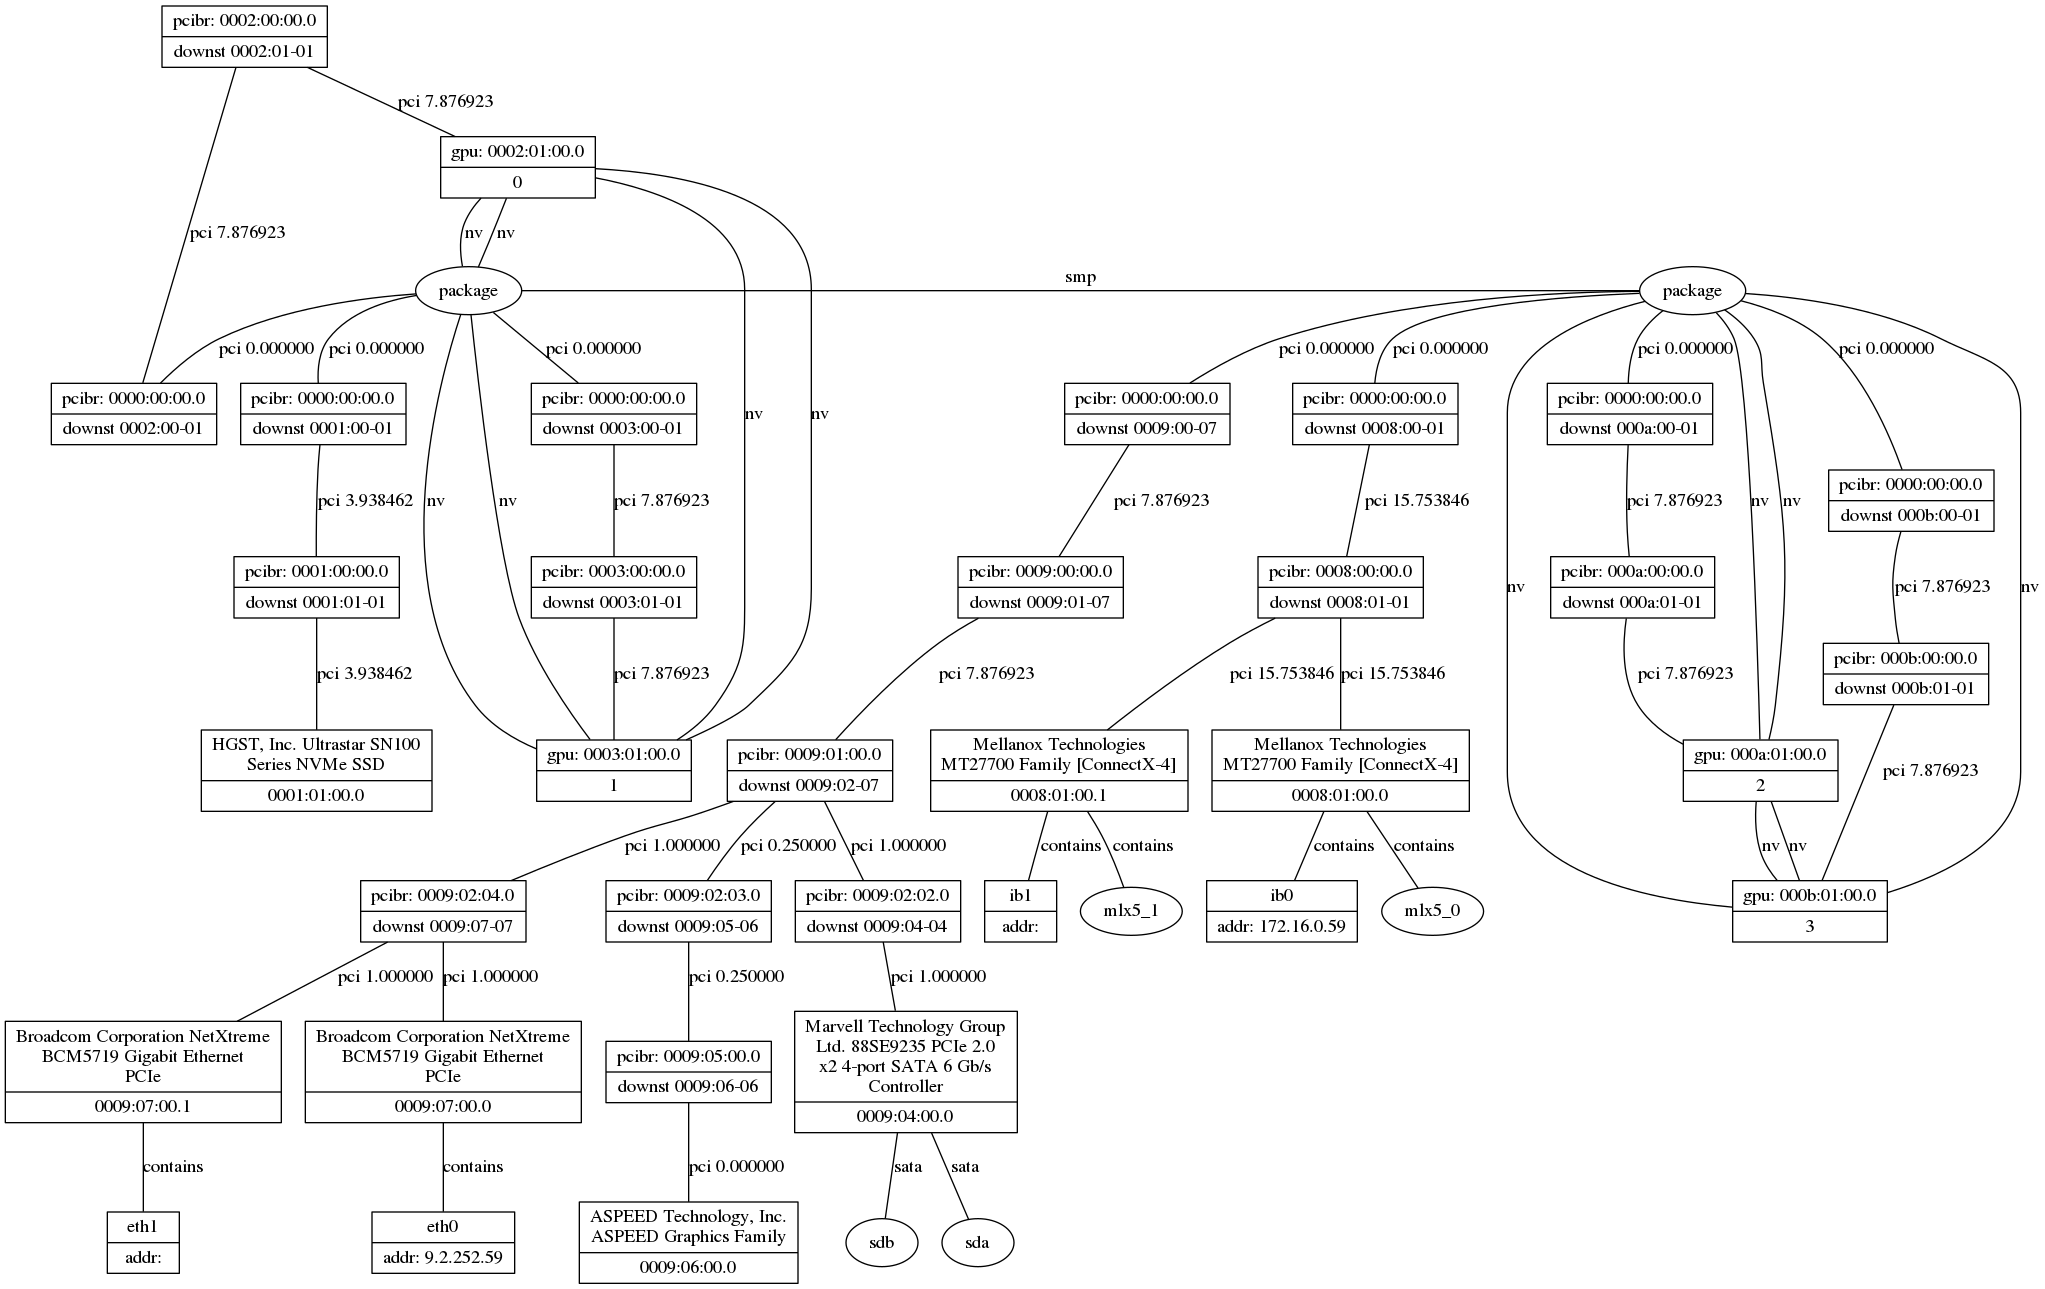
\includegraphics[width=\textwidth]{figures/topo-minsky-actual.png}
    \caption{S822LC discovered topology.}
    \label{fig:topo-minsky-actual}
\end{figure}

\begin{figure}[ht]
    \centering
    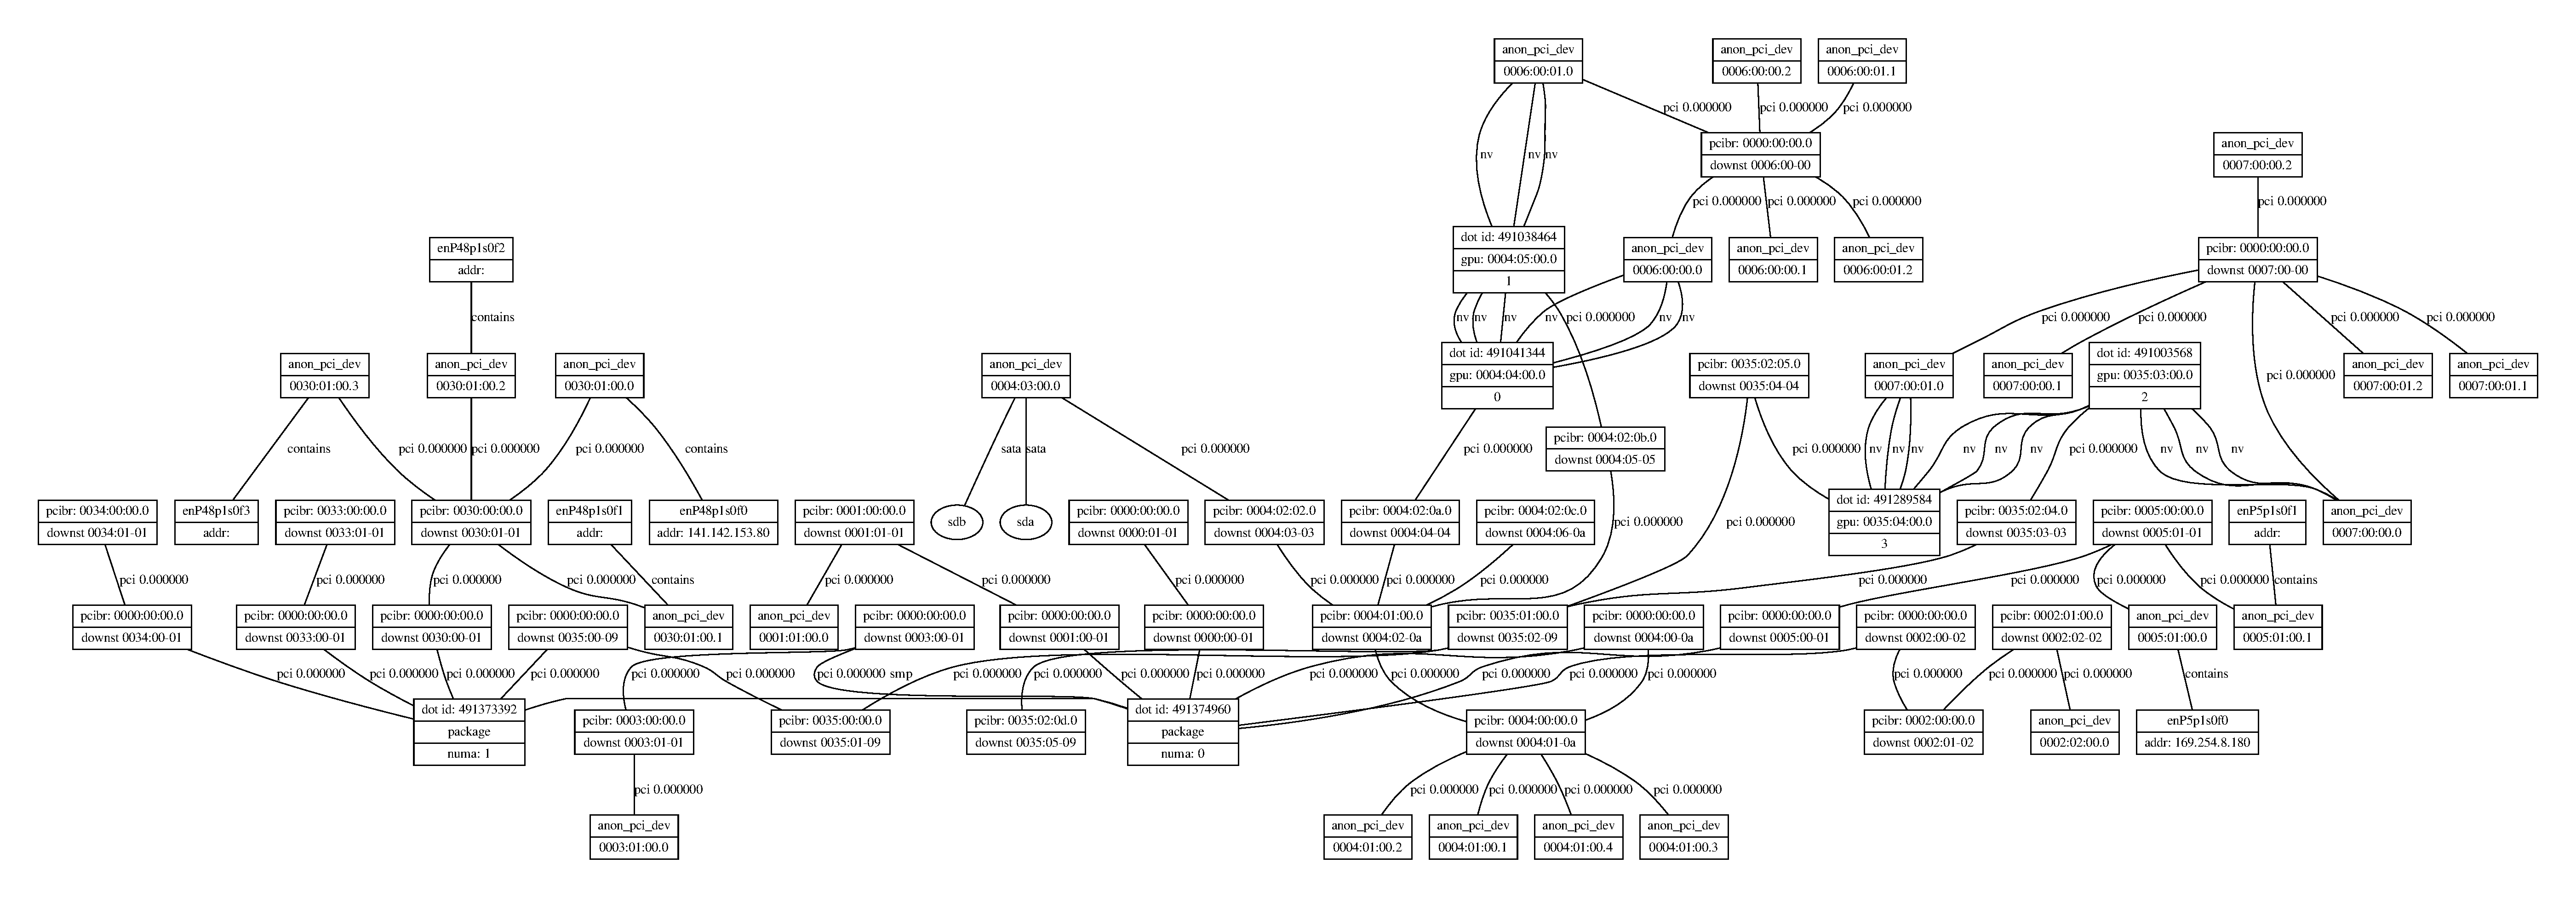
\includegraphics[width=\textwidth]{figures/topo-ac922-actual.pdf}
    \caption{AC922 discovered topology.}
    \label{fig:topo-ac922-actual}
\end{figure}

\begin{figure}[ht]
    \centering
    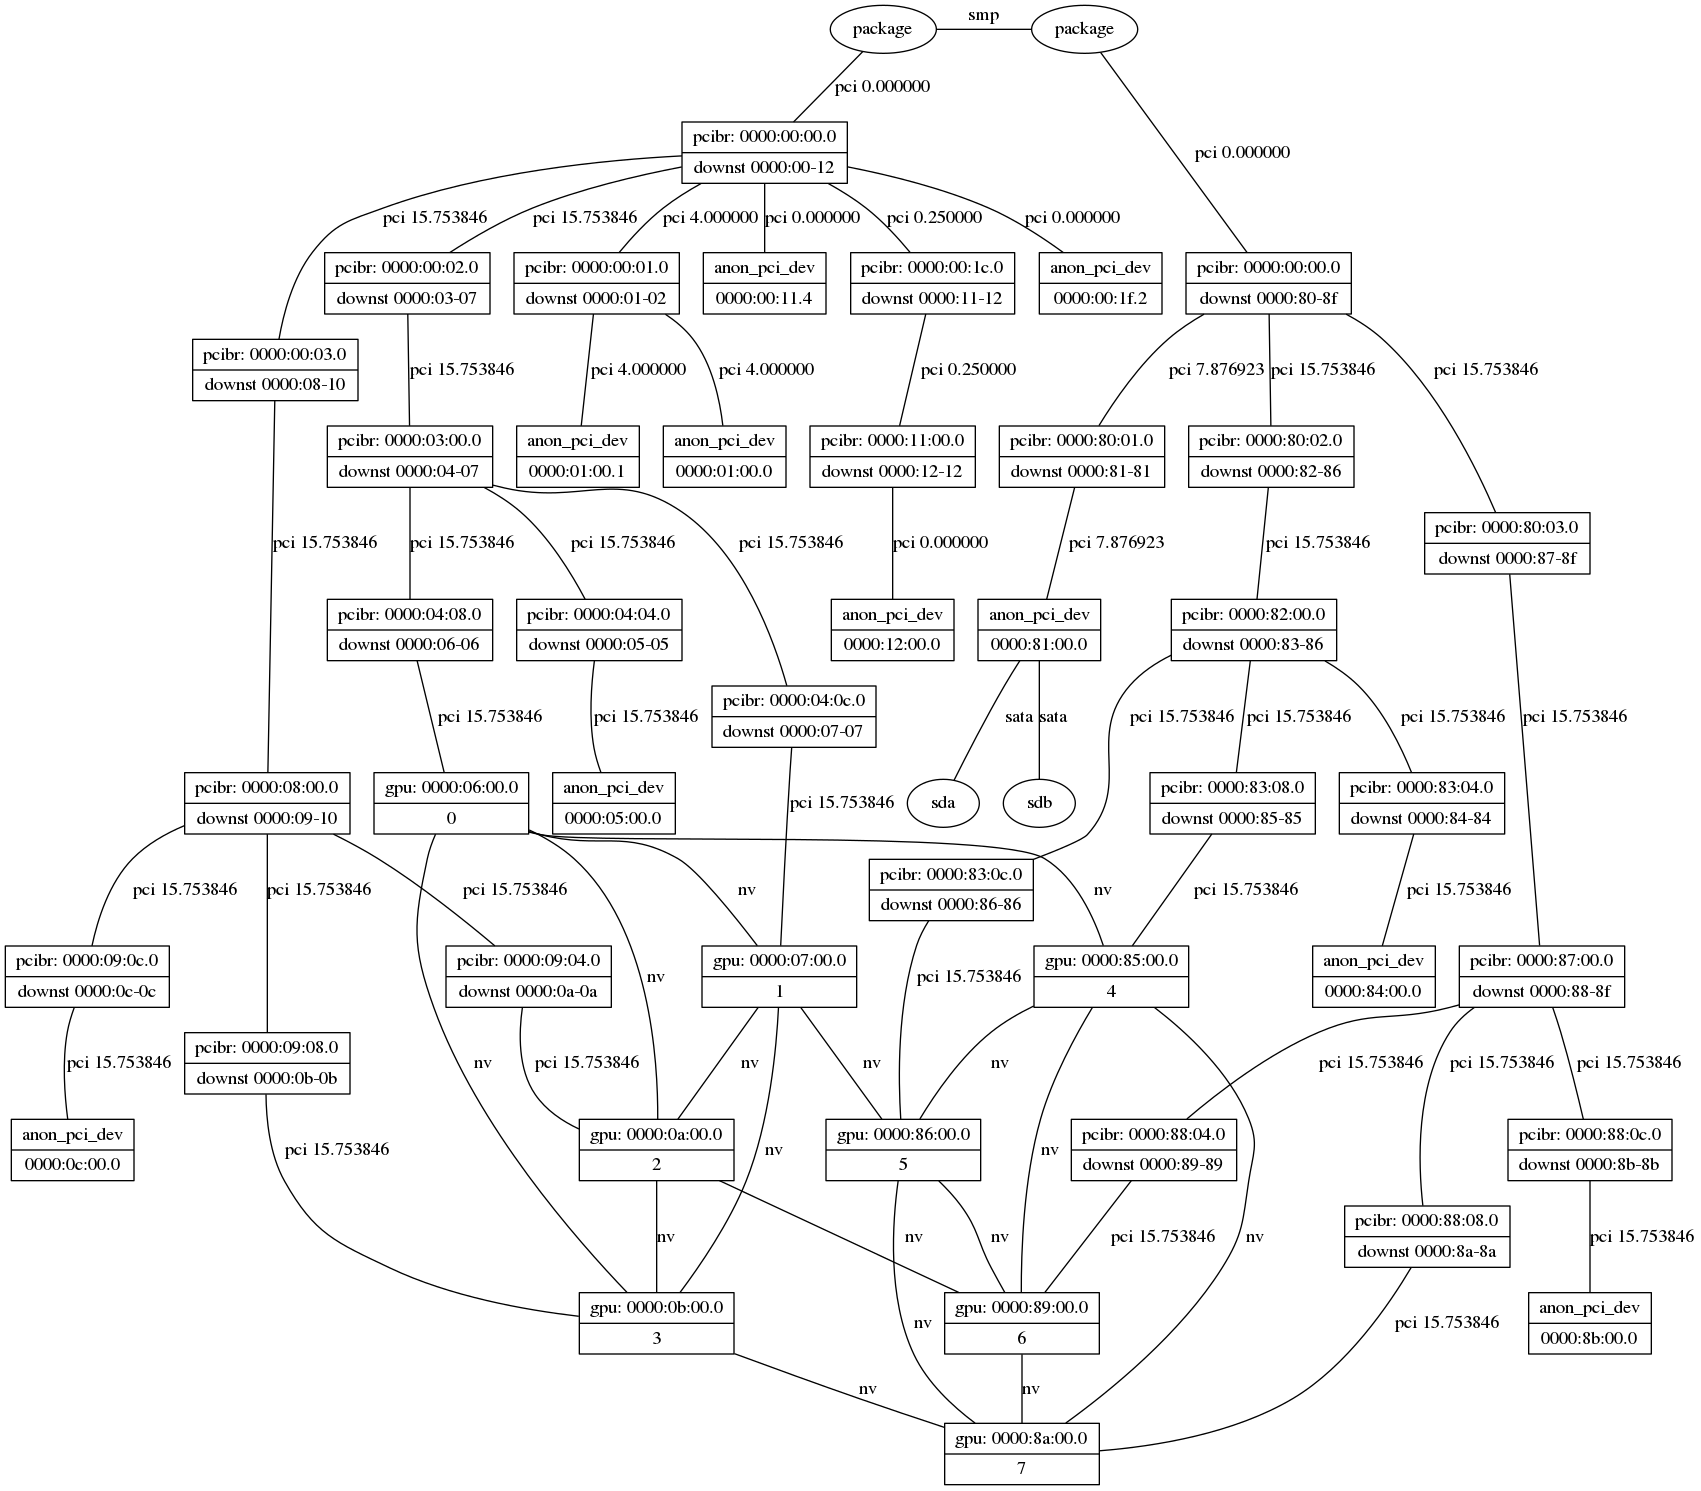
\includegraphics[width=\textwidth]{figures/topo-dgx1-actual.png}
    \caption{DGX-1 discovered topology.}
    \label{fig:topo-dgx-actual}
\end{figure}

\end{appendices}

\backmatter

%%%%%%%%%%%%%%%%%%%%%%%%%%%%%%%%%%%%%%%%%%%%%%%%%%%%%%%%%%%%%%%%%%%%%%%%%%%%%%%
% BIBLIOGRAPHY
%
\bibliographystyle{IEEE_ECE}
% Put references in BibTeX format in thesisrefs.bib.
\bibliography{thesisrefs}


%%%%%%%%%%%%%%%%%%%%%%%%%%%%%%%%%%%%%%%%%%%%%%%%%%%%%%%%%%%%%%%%%%%%%%%%%%%%%%%
% AUTHOR'S BIOGRAPHY
% As of 10/03/2011, Author's Biography or Vita no longer accepted by Grad College

\end{document}
\endinput
